\documentclass[11pt]{article}
\usepackage{hyperref}
\usepackage{listings}
\usepackage{graphicx}
\usepackage{float}
\usepackage{wrapfig}
\usepackage{url}
\title{EECS 433 Project Report: Spiderman - An In-memory Graph Databases}
\author{John Gunderman\\
		Matthew Varley\\
		Umang Banugaria}
\date{}
\begin{document}

\maketitle
\tableofcontents

\section{Introduction}


A graph database is a storage system that stores data using the principles of graph theory. Formally, a graph $G$  is a set of vertices $V$ and a set of edges $E$ such that $G= (V,E)$. Verties of the graph are connected by edges, which can be directed or undirected. An example graph (from the documentation of Neo4j \cite{neo}) is included in Figure \ref{fig:graph}.

\begin{figure}[H]
\centering
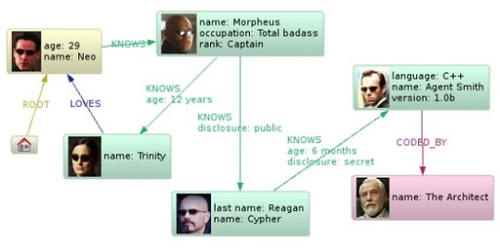
\includegraphics[scale=0.7]{GraphDB.jpg}
\caption{An example graph database from the Matrix\cite{neo}}
\label{fig:graph}
\end{figure}

From the database perspective, a graph database is a storage system that uses index-free adjacency. This means that unlike a relational database, when the user is given a node, there is no need to access an index in order to find all adjacent nodes. Instead, each node in the graph maintains a pointer to its adjacent elements. This makes graph databases excellent for searches that resemble a graph such as RDF data, social networks, or shortest path queries.

In comparison to a relational database, graph databases can handle large datasets easily because queries will not involve join operations. They also are not bound by a rigid schema, which gives graph databases much more flexibility to change and adapt to evolving needs.

Graph databases have become extremely popular over the last few years. The adoption of this technology has been driven largely by companies such as Google, Facebook, and Twitter, each of whom has developed their own graph database frameworks and use them extensively. Twitter uses graph databases to display it’s follower graph. Similarly, Facebook uses graph databases to store their friend graph. Google uses graph databases for their Knowledge Graph \cite{kgraph} technology. They have even developed a tool called Pregel\cite{pregel} which allows them to perform computations across graphs very efficiently.

Over the past two years, graph databases have spread from a niche field to a popular NoSQL option. Many commercial and open source graph databases have flourished because of this. A prime example of such a database is Neo4j\cite{neo}, which is an open source disk-based graph database. Other contenders include GraphDB\cite{graphdb} and FlockDB\cite{flock}. Given the wide range of problems solved by the field of graph databases, we decided to explore this field in our project.

\section{Related Work}

As graph databases have become more widely used, the field has become a growing area of research.  Graph databases have proven to be effective for many applications such a modeling social networks and storing RDF data.  As these datasets become larger, simple querying and storage techniques no longer suffice and therefore significant research has been put into making these databases scalable.  We hope that our contributions will help streamline the research process by providing a base system to work off of.

	A significant portion of the research in the field of graph databases deals with the querying. For example, the k-reach index was introduced in \cite{Cheng} to provide more efficiently execute k-hop reachability queries.  This is the problem of determining if a node can be reached with at most k hops.  The index introduced is based on vertex cover, and is used to assist in querying. The paper concludes that the research it discusses may be the first exploring k-hop reachability queries. The algorithm it presents is meant to serve as a simple solution to the k-hop reachability problem, and should be easily modifiable for future performance gains.

	Another major query type for graph databases is the Steiner tree problem.  This is the problem in graph theory that attempts to find the minimum tree visiting all the nodes in the graph, under certain constraints. In \cite{Star}, a new algorithm, the STAR algorithm, is introduced which solves the Steiner tree problem in better time than any previous solutions: O(log(n)).  The STAR algorithm as introduced in the paper improves upon the BANKS I algorithm, described in the paper. The STAR algorithm has a two stage process. It first scans the graph and creates a spanning tree. It then prunes the tree according to certain heuristics. Based on the experimentation which compares the performance of STAR to other algorithms in the field, it is concluded that the STAR algorithm has better performance in almost all cases.

	In addition to k-hop reachability and Steiner tree problems, the graph database can also be queried as a graph pattern matching problem.  This is the problem of finding subgraphs of the graph database that match a graph pattern with any number of ground instances and variables.  In \cite{Ma}, the method of strong simulation is proposed for the problem of graph pattern matching.  Graph pattern matching is typically described using subgraph isomorphism, however this is an NP-complete problem.  In order to find matches more efficiently, graph simulation is used which has a cubic-time complexity.  Strong simulation is an extension of conventional graph simulation in which duality and locality properties are enforced to obtain better matching results while still maintaining the cubic-time complexity of conventional graph simulation.  Both of these conditions help preserve the topology of data graphs and eliminate excessive matches.  This is just one of the many advancements that have been made in problem of graph pattern matching queries.  Various other advancements in the processing of these queries in social networks have been outlined in \cite{Fan}.

	Beyond just query processing, significant improvements have been made in the way the data is stored to both aid in faster query executions as well as improving the scalability to allow for larger datasets.  In \cite{Sun}, an approach to support subgraph matching without the use if structure indices is described.  The authors point out that all other subgraph matching algorithms rely on indices which can quickly become infeasible for larger graphs as they scale up to one billion nodes due to the superlinear time and space required for index construction.  To avoid using indices, the proposed algorithm would rely on efficient in-memory graph exploration.  Since all the data must be stored in memory, it is split up between machines in a cluster using Trinity, a memory cloud.  With the optimizations and parallel version described in the paper, it was demonstrated that the proposed algorithm could scale up to billion node graphs and it was left as future work to test it on even larger graphs.

	In addition to improving the performance, work has also been done to create new query languages to be able to more easily express more complicated queries.  An example of work done on this front is GraphQL, first introduced in \cite{He}.  GraphQL is a declarative language that uses a graph pattern as the basic operational unit.  It generalizes the selection operator from relational algebra to work with graph pattern matching.

These papers are among the many advancements in graph databases that have been made in the past few years.  However, since graph databases are gaining popularity and the field is still relatively new compared to relational databases, copious amounts of research will be done in the future.  This is where the solution provided in this project comes in.  By providing an easily extensible framework, it can streamline the process of developing and testing new methods in graph databases.

\section{Problem Definition}

The goal of this project was to implement an in-memory graph database. The uses for an in-memory graph database include testing frameworks and high-performance computations. They also perform well at storing semantic data. In this project, we do not try and develop any particularly advanced techniques. Instead we focus on creating research tools that can be helpful in further research in this field. We hope that our project will prove useful for testing new querying techniques and storage data structures.  By providing the basic implementation of a graph database and replaceable components, a new algorithm can be tested by simply swapping out the old module with the newly developed one.

\section{Approach}

We compartmentalized our graph database engine into three main components. These are the storage engine, the relationship definitions, and the query engine. Each of these sections divide again into smaller subcomponents.

\subsection{Storage}

The storage engine, shown in Figure \ref{fig:storage}, currently implements an in-memory datastore for the nodes and relationships of the graph. This could be switched to an on-disk system without a significant amount of effort by taking advantage of the underlying filesystem.

Nodes and relations of the graph are stored in thread-safe, skip-list sets designed for concurrent access inside of an instantiated graph object. This allows multiple operations to be performed on the graph by multiple threads in a safe manner. The sets operate on a “Copy On Write” model where every thread that comes by will receive a common pointer, but will only use a local version (handled invisibly) if the underlying data storage is changed by the query. Once the changed version is committed, any changes are automatically and invisibly merged back into the primary data store. This structure greatly increases the speed of both queries and modifications while preventing conflicts.

A node is stored as a generic container for any type of information. It also contains the set of incoming and outgoing relationships. This allows easy adjacency queries as well as relationship maintenance. Overall, the storage engine for the graph is opaque to the user and can only be accessed through graph and node queries.

\begin{figure}[H]
\centering
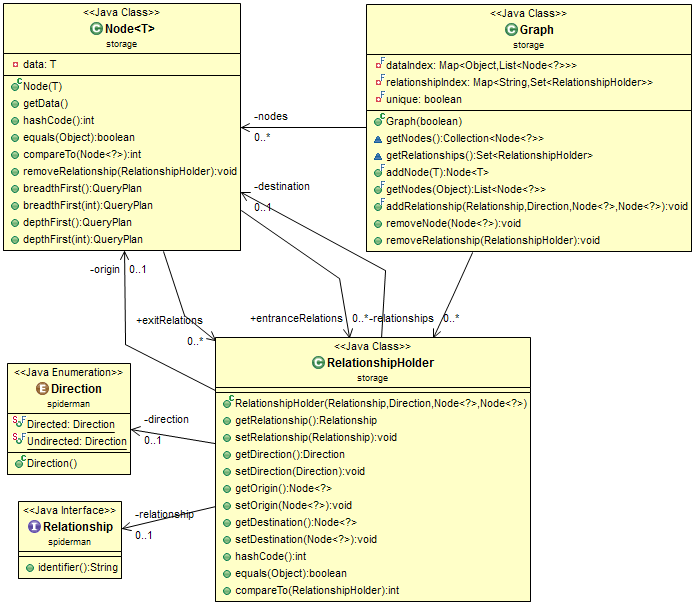
\includegraphics[scale=0.65]{uml.png}
\caption{The storage system class diagram}
\label{fig:storage}
\end{figure}

\subsection{Relationships}

The relationship definitions are an extremely important facet of a working graph database. We have implemented this in our database such that all relationship comparisons are instances of the Relationship interface. This will allow people to define highly modular relationships to suit their needs. For convenience, we have included the NamedRelationship class, which implements the Relationship interface. The NamedRelationship class allows users to name a relationship by string. Other implementations would include data in the class that implements the relationship. This allows a great amount of flexibility, while only requiring the storage engine to know a unique identifier of the relationship (such as the name of the NamedRelationship). This allows queries over only those relationships quickly as the storage engine maintains an index of all relationships by their types.

\subsection{Query Engine}

The query engine is the butter to the storage engine’s bread. With our query engine, we provide two ways to query data from the graph. The first of these is querying the graph proper.

Querying the entire graph is done by bypassing the graph structure. Since we maintain indexes on the nodes and relationships of the graph, we can iterate over these to compute our query result. This tends to be more efficient than a complete graph traversal, as we do not have to look up each objects neighbors at each step before continuing through the graph. Graph queries of this nature must typically involve the entire graph.

The query itself is performed by giving an evaluator object to the graph. Evaluator objects implement the Evaluable interface, which functions similarly to the visitor pattern. The evaluateNode() method of Evaluable is passed each node in turn. If the node should be in the result set, true is returned, and the node will be added to the result set. Otherwise, false is returned.

Localized querying is also important in graph databases. In our implementation, we do this by specifying a start node. Start nodes can be acquired through running a full-graph query, perhaps with a limiter on the number of results returned. They can also be acquired by passing in the known start data as the storage engine maintains a hash index of every node in the graph. 

After a start node is acquired, a query plan can be generated for it. This is done first by specifying whether or not the query will be depth-first or breadth-first. The user can then specify a limit to the results returned, among other options. Finally, an evaluator must be supplied to actually execute the query, as per the full graph queries.

\section{Project Management}

\subsection{Goals of Project}
We aimed to complete the following:

\begin{itemize}
\item Implement a query-able graph datastore for general usage on the local machine.
\item Design sensibly so that a server component could easily be constructed to allow off-site queries of the database.
\item Implement a sensible in-memory storage solution, optimized for graph traversals. The storage API should be modular to allow for different back-ends, including disk and cloud solutions, to be implemented.
\item Implement a query API to allow searches based on node value and the relationships between nodes.
\end{itemize}

These goals have been met.

\subsection{Division of Work}

John - Project Lead, Queries \\
Varley - Storage API, Relationship Definition\\
Umang -  Queries \\


\bibliographystyle{IEEEtran}
\bibliography{bib}

\end{document}
